\documentclass[10pt]{beamer}
\usetheme{Warsaw}
\usecolortheme{dolphin}
\usepackage[utf8]{inputenc}
\usepackage[spanish]{babel}
\usepackage{amsmath}
\usepackage{amsfonts}
\usepackage{amssymb}
\usepackage{graphicx}
\author{Cindy Castellón}
\title[Simulaciones de chubascos con composición mixta]{Simulaciones de chubascos atmosféricos producidos por UHECR con composición mixta}
%\setbeamercovered{transparent} 
\setbeamertemplate{navigation symbols}{} 
%\logo{} 
\institute{Escuela de Física, Universidad de El Salvador} 
%\date{} 
\subject{Proyecto de investigación} 
\begin{document}

\begin{frame}
\titlepage
\end{frame}

\begin{frame}
\tableofcontents
\end{frame}

\section{Marco teórico}

\begin{frame}{Rayos cósmicos}
\begin{figure}
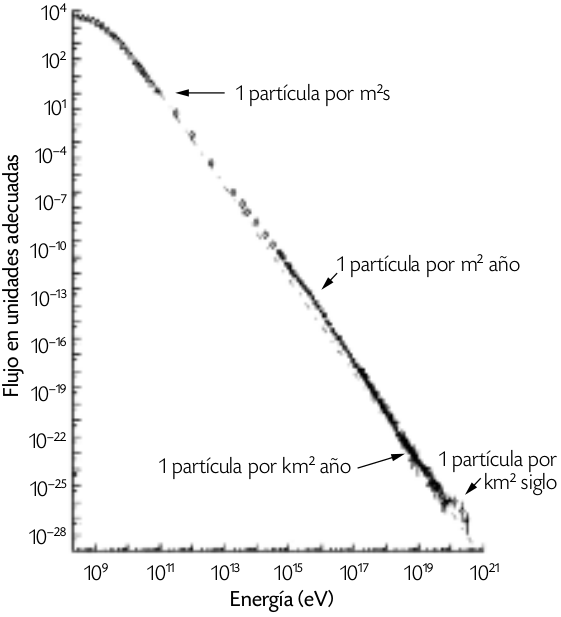
\includegraphics[width=0.5\textwidth]{Figuras/espectro_RC} 
\caption{Intensidad del flujo de rayos cósmicos en función de su energía. Éste está bien representado por una ley de potencias $E^{-2.7}$. (Tomada de \cite{Poderosas})}
\end{figure}
\end{frame}

\begin{frame}{Chubascos atmosféricos}
\begin{figure}
	\centering
	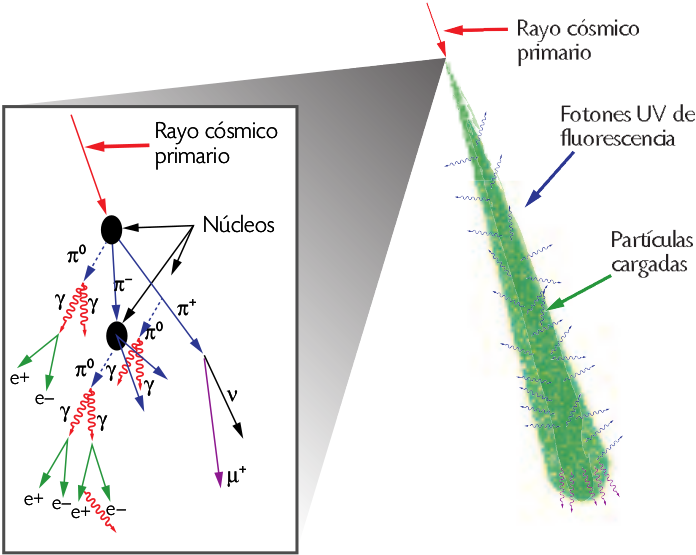
\includegraphics[width=0.7\textwidth]{Figuras/air_shower} 
	\caption{Esquema de la formación y desarrollo de un chubasco atmosférico. Se observa la componente hadrónica y la electromagnética. (Tomada de \cite{Poderosas})}
	\label{fig:airshower}
	\end{figure}	
\end{frame}

\begin{frame}{Estado del conocimiento}
\begin{figure}
\centering
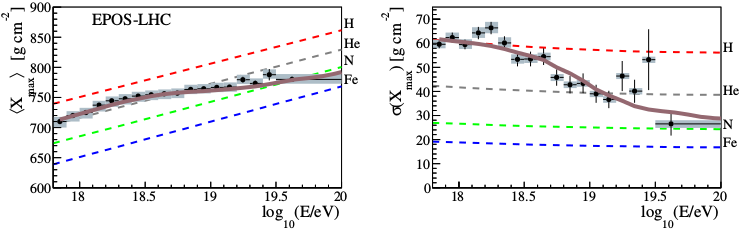
\includegraphics[width=0.95\textwidth]{Figuras/Xmax_PAO} 
\caption{$X_{max}$ promedio (izquierda) y desviación estándar (derecha) asumiendo una composición mixta (línea sólida), comparado con datos del PAO \cite{PAOcomposition}.}
\label{fig:Xmax}
\end{figure}	
\end{frame}

\begin{frame}
\begin{figure}
\centering
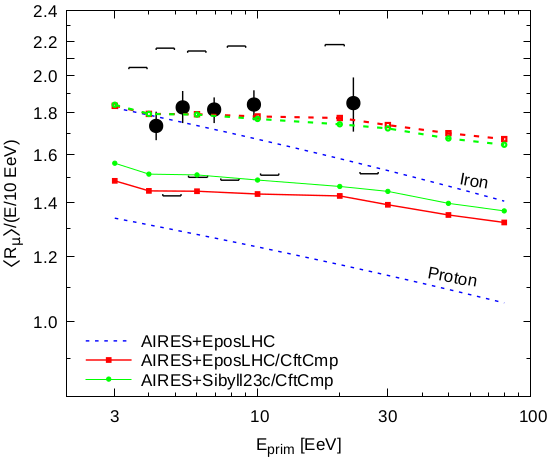
\includegraphics[width=0.6\textwidth]{Figuras/Nmu_Sciutto} 
\caption{Las líneas sólidas verde y roja corresponden a la estimación del número de muones utilizando el sistema AIRES con diferentes modelos hadrónicos. Se observa que al desplazarlas una constante éstas tienen buena concordarcia con los datos experimentales (círculos negros) \cite{Sciutto2019}.}
\label{fig:Nmu}
\end{figure}	
\end{frame}

\section{Planteamiento del problema}

\begin{frame}{Preguntas de investigación}
\begin{itemize}
\item ¿Cómo afecta la composición del flujo de UHECR a la distribución lateral de electrones y de muones? \vspace{0.3 cm}
\item ¿la distribución lateral de electrones y muones obtenida en simulaciones es sensible al modelo de interacciones hadrónicas utilizado? \vspace{0.3 cm}
\item ¿los resultados de la distribución lateral apoyan la hipótesis de una composición primaria mixta? y \vspace{0.3 cm}
\item ¿la composición mixta deducida a partir de otras observables es congruente con los resultados y mediciones de la distribución lateral?
\end{itemize}
\end{frame}

\begin{frame}{Objetivo general}
Estudiar el efecto de una composición primaria mixta de los UHECR en la distribución lateral de electrones y muones, con el fin de observar si la composición primaria que se ha obtenido por la colaboración Pierre Auger, a partir de mediciones de la profundidad de máximo y el número de muones, es consistente con otras observables de los chubascos.
\end{frame}

\begin{frame}{Objetivos específicos}

\begin{enumerate}
\item Verificar el efecto de una composición mixta de los UHECR en las observables $X_{\text{max}}$ y $\sigma X_{\text{max}}$ realizando simulaciones de chubascos atmosféricos con el sistema AIRES y comparando con resultados publicados por la colaboración Pierre Auger.\vspace{0.3 cm}
	
	\item Analizar las distribuciones laterales de electrones y muones en chubascos producidos por rayos cósmicos de composición mixta. \vspace{0.3 cm}
	
	\item Examinar las discrepancias entre las predicciones de las distribuciones laterales realizadas con los diferentes modelos hadrónicos de altas energías disponibles en AIRES. \vspace{0.3 cm}
	
	\item Comparar los resultados de las distribuciones laterales obtenidos de las simulaciones con los respectivos datos tomados por el Observatorio Pierre Auger. \vspace{0.3 cm}
\end{enumerate}
\end{frame}

\begin{frame}{Justificación}
Deficiencias en el conocimiento del tema: \vspace{0.5 cm}
\begin{itemize}
\item Existen discrepancias entre predicciones de diferentes modelos hadrónicos. \vspace{0.5 cm}
\item No coinciden las simulaciones de chubascos atmosféricos producidos por UHECR con las observaciones. \vspace{0.5 cm}
\item La colaboración Pierre Auger ha propuesto una composición mixta de los UHECR.
\end{itemize}
\end{frame}

\begin{frame}

Esta investigación pretende estudiar los efectos de la composición de los UHECR en diferentes observables del desarrollo de chubascos atmosféricos mediante simulaciones, se busca apoyar o contradecir la hipósisis de una composición mixta de los UHECR. \\ \vspace{0.6 cm}

Asimismo se quiere analizar la sensibilidad de los resultados de las distribuciones laterales al modelo de interacción hadrónica, para potencialmente sugerir el empleo de estos observables en nuevos estudios acerca de la composición primaria de rayos cósmicos.
\end{frame}

\begin{frame}{Viabilidad}
\begin{itemize}
\item El sistema AIRES es de acceso libre y está disponible en línea en el sitio \url{http://aires.fisica.unlp.edu.ar/}. \vspace{0.5 cm}
\item Se han realizado ejecuciones de prueba en una computadora personal para estimar el tiempo de simulación. \vspace{0.5 cm}
\item Datos del Observatorio Pierre Auger están publicados en su repositorio en el sitio web. \vspace{0.5 cm}
\item La asesora principal del proyecto, PhD. Karen Caballero, es parte de la colaboración Pierre Auger, siendo su especialidad la física de astropartículas.
\end{itemize}

\end{frame}

\section{Metodología}
\begin{frame}{Metodología}
Con el sistema AIRES se simularán chubascos producidos por rayos cósmicos de energías entre $10^{17.256}$ y $10^{19.626}$ eV, en la ubicación de Malargue en Mendoza, Argentina -donde se encuentra una de las estaciones del PAO-. \\ \vspace{0.5 cm}

Se considerarán direcciones de incidencia con ángulo zenital entre 0$^{o}$ y 70$^{o}$ y ángulo azimutal distribuido isotrópicamente entre 0$^{o}$ y 360$^{o}$. \\ \vspace{0.5 cm}

Se utilizarán tres modelos de interacciones hadrónicas de altas energías; Sibyll 2.3c, EPOS-LHC y QGSJETII-04.
\end{frame}

\begin{frame}
\begin{figure}[h]
\centering
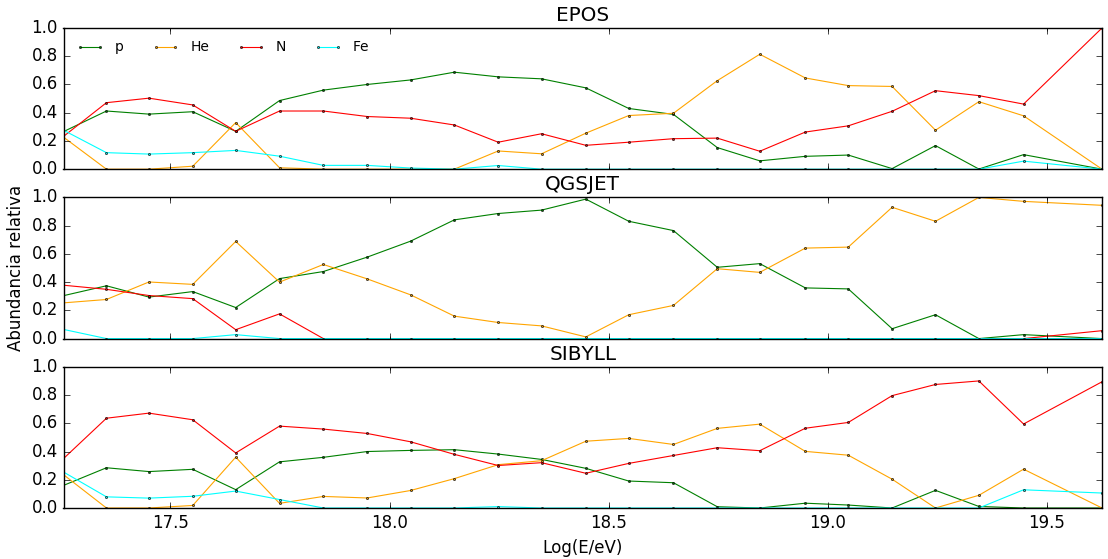
\includegraphics[height=0.6\textheight]{Figuras/composition} 
\caption{Composición en función de la energía, resultado de ajustes con los datos de $X_{\text{max}}$ del Observatorio Pierre Auger realizados con tres modelos de interacciones hadrónicas de altas energías.}
\label{fig:composition}
\end{figure}	
\end{frame}

\begin{frame}
En síntesis, el sistema AIRES consiste de:\vspace{0.3 cm}
	\begin{itemize}
	\item Los programas de simulación principales (AiresEPLHC, AiresEP199, AiresQIIr03, AiresQIIr04, AiresS21, AiresS23, AiresS23c), cada uno conteniendo la interfaz para un paquete de interacciones hadrónicas. \vspace{0.3 cm}
	\item El programa resumen (AiresSry), diseñado para procesar parte de los datos generados por los programas de simulación. \vspace{0.3 cm}
	\item El programa de conversión de formato IDF (\textit{internal dump file}) a ADF (\textit{portable dump file}) (AiresIDF2ADF). \vspace{0.3 cm}
	\item Una librería de auxiliares para procesar los archivos de salida de los programas de simulación (libAires.a). \vspace{0.3 cm}
	\item El \textit{AIRES runner system}, para facilitar el trabajo con AIRES en ambientes UNIX. \vspace{0.3 cm}
	\end{itemize}
\end{frame}

\section{Cronograma de actividades}

\begin{frame}{Cronograma de actividades}

\begin{footnotesize}
\begin{table}
\bgroup
\def\arraystretch{1.5}
\begin{tabular}{|l|l|}
\hline
\multicolumn{1}{|c|}{\textbf{ACTIVIDAD}}                                            & \multicolumn{1}{c|}{\textbf{FECHAS}} \\ \hline

Creación de archivos de \textit{input} especificando \\los parámetros de las simulaciones.						& 18/sep - 21/sep			\\ \hline	
Solicitud de datos observacionales del \\Observatorio Pierre Auger.         									& sep                         \\ \hline
Simulación de chubascos producidos por protones \\de $10^{17}$ a $10^{20}$ eV con el modelo SYBILL. 				& 21/sep - 27/sep             \\ \hline
Simulación de chubascos producidos por núcleos de hierro \\ de $10^{17}$ a $10^{20}$ eV con el modelo SYBILL. 	& 28/sep - 04/oct             \\ \hline
Simulación de chubascos con composición mixta \\de $10^{17}$ a $10^{20}$ eV con el modelo SYBILL.   				& 05/oct - 11/oct             \\ \hline
Realizar gráficas de $X_{max}$, $\sigma X_{max}$, \\y distribuciones laterales de las simulaciones con SYBILL.	& 12/oct  		              \\ \hline
Validación de resultados de SYBILL.              																& 13/oct - 16/oct             \\ \hline

\end{tabular}
\egroup
\end{table}
\end{footnotesize}
\end{frame}

\begin{frame}{Cronograma de actividades}

\begin{footnotesize}
\begin{table}
\bgroup
\def\arraystretch{1.5}
\begin{tabular}{|l|l|}
\hline
\multicolumn{1}{|c|}{\textbf{ACTIVIDAD}}                                            & \multicolumn{1}{c|}{\textbf{FECHAS}} \\ \hline
Comparación entre resultados de SYBILL con \\distintas composiciones. 											& 17/oct - 20/oct			 \\ \hline
Simulación de chubascos producidos por protones \\de $10^{17}$ a $10^{20}$ eV con el modelo EPOS. 				& 12/oct - 18/oct             \\ \hline
Simulación de chubascos producidos por núcleos de hierro \\de $10^{17}$ a $10^{20}$ eV con el modelo EPOS. 		& 19/oct - 25/oct             \\ \hline
Simulación de chubascos con composición mixta \\de $10^{17}$ a $10^{20}$ eV con el modelo EPOS.   				& 26/oct - 01/nov             \\ \hline
Realizar gráficas de $X_{max}$, $\sigma X_{max}$, \\y distribuciones laterales de las simulaciones con EPOS.		& 02/nov  		              \\ \hline
Validación de resultados de EPOS.              																& 03/nov - 06/nov             \\ \hline
Comparación entre resultados de EPOS con \\distintas composiciones.              								& 07/nov - 10/nov             \\ \hline
\end{tabular}
\egroup
\end{table}
\end{footnotesize}
\end{frame}

\begin{frame}{Cronograma de actividades}

\begin{footnotesize}
\begin{table}
\bgroup
\def\arraystretch{1.5}
\begin{tabular}{|l|l|}
\hline
\multicolumn{1}{|c|}{\textbf{ACTIVIDAD}}                                            							& \multicolumn{1}{c|}{\textbf{FECHAS}} \\ \hline
Simulación de chubascos producidos por protones de\\ $10^{17}$ a $10^{20}$ eV con el modelo QGSJET. 				& 02/nov - 08/nov             \\ \hline
Simulación de chubascos producidos por núcleos de hierro de\\ $10^{17}$ a $10^{20}$ eV con el modelo QGSJET. 	& 09/nov - 15/nov             \\ \hline
Simulación de chubascos con composición mixta de \\$10^{17}$ a $10^{20}$ eV con el modelo QGSJET.  				& 16/nov - 22/nov             \\ \hline
Realizar gráficas de $X_{max}$, $\sigma X_{max}$, \\y distribuciones laterales de las simulaciones con QGSJET.	& 23/nov 		              \\ \hline
Validación de resultados de EPOS.              																& 24/nov - 27/nov             \\ \hline
Comparación entre resultados de QGSJET con \\distintas composiciones.              								& 28/nov - 01/dic             \\ \hline
Comparación entre resultados de los tres modelos hadrónicos.     												& 02/dic - 05/dic             \\ \hline
Comparación entre simulaciones y observaciones.																& 06/dic - 09/dic             \\ \hline
\end{tabular}
\egroup
\end{table}
\end{footnotesize}
\end{frame}

\end{document}